\section{System Availability Managers }\label{system-availability-managers}

\subsection{Overview}\label{overview-025}

System availability managers, or AvailabilityManagers, are one of the high-level control constructs in EnergyPlus. An AvailabilityManager is able to access data from any of the HVAC system nodes and use this data to set flags telling a central air system or plant loop to turn on or off. Also, some of the HVACZone:* components can use these same availability managers to turn their supply air fan on or off. Each type of availability manager encapsulates a specific high-level on-off control strategy. For instance, the input object AvailabilityManager:NightVentilation allows the user to specify a control strategy for pre-cooling the building with night-time ventilation.

Availability managers are contained in the program module \emph{SystemAvailabilityManager}. The Availability managers are executed at the start of each HVAC time step by a call to \emph{ManageSystemAvailability}, and they reside outside the HVAC system iteration loops. Thus, the availability managers are executed once per HVAC time step, and they use previous time step information to calculate their control actions.

If a given instance of an AvailabilityManager is specific to an AirLoopHVAC or to a PlantLoop, then in the input, each loop references its availability managers through a AvailabilityManagerAssignmentList. Once the data has been read in and processed, the AvailabilityManager data for each loop is stored in array \emph{PriAirSysAvailMgr} in \emph{DataAirLoop} (for AirLoopHVAC) and in array \emph{PlantAvailMgr} ~in \emph{DataPlant} for plant loops.

The availability status for each AirLoopHVAC (\emph{PriAirSysAvailMgr}) is also passed to a zone equipment availability status array (\emph{ZoneEquipAvail}) for possible use by the zones served by that air loop. This sets the availability for certain zone equipment which are assumed to operate in conjunction with the air loop. Specifically, the availability of zone exhaust fans (Ref. Fan:ZoneExhaust) and terminal unit fans (Ref. AirTerminal:SingleDuct:SeriesPIU: Reheat, AirTerminal:SingleDuct: ParallelPIU:Reheat, and AirTerminal:SingleDuct:VAV: Reheat:VariableSpeedFan), if specified in the input, will be the same as the corresponding AirLoopHVAC availability if an AvailabilityManager is specified. Other zone equipment are not affected by the AirLoopHVAC system availability managers (e.g., Window AC, PTAC and PTHP).

However, system availability managers can separately be specified for zone components (currently only allowed for Window AC, PTAC, PTHP, Unit Heater, Unit Ventilator, Zone Water to Air Heat Pump, Zone Terminal Unit (VRF), Standalone Energy Recovery Ventilator, Outdoor Air Unit, Fan Coil Unit, and Ventilated Slab). Similar to AirLoopHVAC or PlantLoop, inputs of these zone components refer to their availability managers through a AvailabilityManagerAssignmentList. System availability managers only operate when zone components are available. If the Window AC (or any other unit) is scheduled off then the system availability manager will not operate until the Window AC is scheduled on. The functioning of the system availability manager for zone components is same as for AirLoopHVAC or PlantLoop. Except night ventilation SAM, all other SAMs can be specified for these zone components.

The actual action of turning on or off a loop is taken by the loop prime movers: fans for AirLoopHVACs and pumps for plant loops. For instance when a fan is deciding whether it is on or off, it checks its on/off schedule and whether the loop availability status flag is \emph{CycleOn} or \emph{ForceOff}. If the schedule is on and the status flag is \emph{ForceOff}, the fan will be off. If the fan schedule says off and the status flag is \emph{CycleOn}, the fan will be on. Thus the availability managers overrule the fan on/off schedule.

\subsection{Scheduled}\label{scheduled-000}

The input object AvailabilityManager:Scheduled provides the simplest availability manager. The sole input for this manager is a schedule name. If the current schedule value is \textgreater{} 0.0, the availability status flag is set to \emph{CycleOn}; otherwise it is set to \emph{ForceOff}.

\subsection{Scheduled On}\label{scheduled-on}

An alternative to the AvailabilityManager:Scheduled object is the \emph{AvailabilityManager:ScheduledOn} that is used specifically to turn equipment on while other availability managers may be used to turn the equipment off. The sole input for this manager is a schedule name. If the current schedule value is \textgreater{} 0.0, the availability status flag is set to \emph{CycleOn}; otherwise it is set to \emph{NoAction}.

\subsection{Scheduled Off}\label{scheduled-off}

An alternative to the AvailabilityManager:Scheduled object is the \emph{AvailabilityManager:ScheduledOff} that is used specifically to turn equipment off while other availability managers may be used to turn the equipment on. The sole input for this manager is a schedule name. If the current schedule value is = 0.0, the availability status flag is set to \emph{ForceOff}; otherwise it is set to \emph{NoAction}.

\subsection{Night Cycle}\label{night-cycle}

The input object AvailabilityManager:NightCycle is to specify when a system that has been scheduled off during unoccupied hours should cycle on to prevent building temperatures from becoming too hot or too cold. This manager can not be used to force a system off. The inputs are:

\begin{itemize}
\item  A manager applicability schedule;

\item  The name of the fan schedule this manager will override;

\item  The control type: \emph{StayOff}, \emph{CycleOnAny}, \emph{CycleOnControlZone}, \emph{CycleOnAnyZoneFansOnly} \emph{CycleOnAnyCoolingOrHeatingZone}, \emph{CycleOnAnyCoolingZone}, \emph{CycleOnAnyHeatingZone}, or \emph{CycleOnAnyHeatingZoneFansOnly};

\item  Thermostat on/off tolerance \emph{T\(_{tol}\)} (\(^{\circ}\)C);

\item  Cycling run time control type: \emph{FixedRunTime}, \emph{Thermostat}, or \emph{ThermostatWithMinimumRunTime};

\item  Cycling run time in seconds; used to calculate a stop time (in time steps since the start of the current run period) once the status has become \emph{Cycle On}.

\item  A control zone or zone list name.

\item  Cooling control zone or zone list name.

\item  Heating control zone or zone list name.

\item  Heating zone fans only control zone or zone list name.

\end{itemize}

If the fan schedule current value is \textgreater{} 0 or the applicability schedule value is \(\le\) ~0 , \emph{AvailStatus = NoAction}.

If the program is in warmup, the start time stop time are reset to the current time.

Otherwise:

\begin{enumerate}
\item  If current time (in time steps since the start of the run period) is greater than the start time and less than the stop time, \emph{AvailStatus = CycleOn} (or \emph{CycleOnZoneFansOnly} if the control type is \emph{Cycle On Any -- Zone Fans only}) for CyclingRunTimeControlType = \emph{CyclingRunTimeControlType = FixedRunTime}, or \emph{CyclingRunTimeControlType = ThermostatWithMinimumRunTime} but for \emph{CyclingRunTimeControlType = Thermostat} the availability status is determined based on the zone air and the thermostat setpoint temperature difference and the tolerance limits.  

\item  If the current time equals the stop time and the CyclingRunTimeControlType = \emph{CyclingRunTimeControlType = FixedRunTime}, or \emph{CyclingRunTimeControlType = ThermostatWithMinimumRunTime}, \emph{AvailStatus = NoAction} ~and the fan schedule will determine if the system is on. For \emph{CyclingRunTimeControlType = Thermostat} the availability status is determined based on the zone air and the thermostat setpoint temperature difference and the tolerance limits, and the fan schedule will determine if the system is on.

\item  If the current time is greater than the stop time, the manager can potentially cycle the system on for \emph{CyclingRunTimeControlType = FixedRunTime}, \emph{CyclingRunTimeControlType = Thermostat}, or \emph{CyclingRunTimeControlType = ThermostatWithMinimumRunTime}.

  \begin{enumerate}
  \item  For control types \emph{CycleOnAny} and \emph{CycleOnAnyZoneFansOnly} the manger looks at each zone served by the air loop and detects whether the zone temperature at the thermostat is greater than the cooling setpoint plus ½\emph{T\(_{tol}\)} or less than the heating setpoint minus ½\emph{T\(_{tol}\)}. If it is, \emph{AvailStatus} is set to \emph{CycleOn} (or \emph{CycleOnZoneFansOnly}). If not, \emph{AvailStatus} is set to \emph{NoAction}.

  \item  For control type \emph{CycleOnControlZone}, the manager does the same check just for the control zone or zone list.

  \item  For control type \emph{CycleOnAnyCoolingOrHeatingZone}, the manager checks the cooling setpoint for the cooling control zone or zone list and sets \emph{AvailStatus} to \emph{CycleOn}, then it checks the heating setpoint for the heating control zone or zone list and sets \emph{AvailStatus} to \emph{CycleOn}. If the \emph{AvailStatus} is still \emph{NoAction}, then the manager checks the heating setpoint for the heating zone fans only zone or zone list and sets \emph{AvailStatus} to \emph{CycleOnZoneFansOnly}). If none of these checks are true then \emph{AvailStatus} is set to \emph{NoAction}.

  \item  For control type \emph{CycleOnAnyCoolingZone}, the manager checks the cooling setpoint for the cooling control zone or zone list and sets \emph{AvailStatus} to \emph{CycleOn}. If none of these checks are true then \emph{AvailStatus} is set to \emph{NoAction}.

  \item  For control type \emph{CycleOnAnyHeatingZone}, the manager checks the heating setpoint for the heating control zone or zone list and sets \emph{AvailStatus} to \emph{CycleOn}. If the \emph{AvailStatus} is still \emph{NoAction}, then the manager checks the heating setpoint for the heating zone fans only zone or zone list and sets \emph{AvailStatus} to \emph{CycleOnZoneFansOnly}). If none of these checks are true then \emph{AvailStatus} is set to \emph{NoAction}.

  \item  For control type \emph{CycleOnAnyHeatingZoneFansOnly}, the manager checks the heating setpoint for the heating zone fans only zone or zone list and sets \emph{AvailStatus} to \emph{CycleOnZoneFansOnly}). If none of these checks are true then \emph{AvailStatus} is set to \emph{NoAction}.

  \end{enumerate}

\item  Lastly if the new status is CycleOn the start time is reset to the current time and the stop time is reset. When this availability manager is specified for a zone component then the only allowed control types are \emph{StayOff} \emph{and} \emph{CycleOnControlZone.}
\end{enumerate}

\subsection{Night Ventilation}\label{night-ventilation}

The input object AvailabilityManager:NightVentilation is a manager that looks at indoor and outdoor conditions to see if night ventilation might be beneficial. In addition to being able to cycle the air system on, this manager can specify what the ventilation air flow rate should be.~ The inputs are:

\begin{itemize}
\item A manager applicability schedule;
\item The name of the fan schedule this manager will override;
\item A ventilation temperature schedule;
\item A ventilation delta T;
\item A ventilation low limit temperature;
\item The night ventilation flow fraction;
\item The name of the control zone.
\end{itemize}

If the fan schedule current value is \textgreater{} 0 or the applicability schedule value is \(\le\) 0 or if the program is in warmup, \emph{AvailStatus = NoAction}.

Otherwise, the manager performs 3 limit checks.

\begin{enumerate}
\item If for all the zones connected to the air loop the room temperature at the thermostat of any zone is greater than the ventilation temperature schedule value, this check is true.
\item If for all the zones connected to the air loop the room temperature at the thermostat of any zone is less than the ventilation low limit temperature, this check is true.
\item If the difference between the control zone room temperature at the thermostat and the outside temperature is greater than the specified night venting delta T, this check is true.
\end{enumerate}

If 1) and 3) are true and 2) is false, the status is set to \emph{CycleOn}; otherwise the status is \emph{NoAction}.~ If the status is \emph{CycleOn} this manager sets some additional values in the \emph{AirLoopControlInfo} data structure (a flag is set to indicate night ventilation is occurring and a flag is set to indicate that the air system flow rate has been specified by a manager) and in the \emph{~AirLoopFlow} data structure (the system flow fraction is specified). The night ventilation flag indicates to the fan that it should use alternate performance characteristics if they have been specified in a FanPerformance:NightVentilation object.

\subsection{Differential Thermostat}\label{differential-thermostat}

The input object AvailabilityManager:DifferentialThermostat is a manager that overrides fan or pump schedules depending on the temperature difference between two nodes. A typical use would be for one node to be an outdoor air node and the other a zone node. The inputs are:

\begin{itemize}
\item name of the hot node;
\item name of the cold node;
\item temperature difference for turning the system on (\emph{DeltaT\(_{on}\)});
\item temperature difference for turning the system off (\emph{DeltaT\(_{off}\)}).
\end{itemize}

As shown by the following pseudo code, there is no applicability schedule for this manager. Also, this manager always returns a status of \emph{CycleOn} or \emph{ForceOff}, never \emph{NoAction}.

\emph{DeltaT} = \emph{T\(_{hot~node}\)} -- \emph{T\(_{cold~node}\)}

If \emph{DeltaT} \textgreater{} = \emph{DeltaT\(_{on}\)} then

~~~~\emph{AvailStatus = CycleOn}

Else if \emph{DeltaT} \textless{} = \emph{DeltaT\(_{off}\)} then

~~~~\emph{AvailStatus = ForceOff}

Else

~~~~\emph{AvailStatus} remains in its previous state.

End If

\subsection{High Temperature Turn Off}\label{high-temperature-turn-off}

The input object AvailabilityManager:HighTemperatureTurnOff is used to turn off a central air system or a plant loop if a sensed node temperature exceeds a temperature limit. The inputs are:

\begin{itemize}
\item name of the sensed node;
\item limit temperature (\emph{T\(_{u}\)}).
\end{itemize}

In pseudo code:

If \emph{T\(_{sensed~node}\)} \textgreater{} = \emph{T\(_{u}\)} then

~~~~\emph{AvailStatus} = \emph{ForceOff}

Else

~~~~\emph{AvailStatus} = \emph{NoAction}

End If

\subsection{High Temperature Turn On}\label{high-temperature-turn-on}

The input object AvailabilityManager:HighTemperatureTurnOn is used to turn on a central air system or a plant loop if a sensed node temperature exceeds a temperature limit. The inputs are:

\begin{itemize}
\item name of the sensed node;
\item limit temperature (\emph{T\(_{u}\)}).
\end{itemize}

In pseudo code:

If \emph{T\(_{sensed~node}\)} \textgreater{} = \emph{T\(_{u}\)} then

~~~~\emph{AvailStatus} = \emph{CycleOn}

Else

~~~~\emph{AvailStatus} = \emph{NoAction}

End If

\subsection{Low Temperature Turn Off}\label{low-temperature-turn-off}

The input object AvailabilityManager:LowTemperatureTurnOff is used to turn off a central air system or a plant loop if a sensed node temperature is lower than a temperature limit. The inputs are:

\begin{itemize}
\item name of the sensed node;
\item limit temperature (\emph{T\(_{l}\)});
\item applicability schedule name.

\end{itemize}

If the applicability schedule exists and has a current value of \textless{} = 0, the manager returns an availability status of \emph{NoAction}.

Otherwise, as shown by the following pseudo code:

If \emph{T\(_{sensed~node}\)} \textless{} = \emph{T\(_{l}\)} then

~~~~\emph{AvailStatus} = \emph{ForceOff}

Else

~~~~\emph{AvailStatus} = \emph{NoAction}

End If

\subsection{Low Temperature Turn On}\label{low-temperature-turn-on}

The input object AvailabilityManager:LowTemperatureTurnOn is used to turn on a central air system or a plant loop if a sensed node temperature is less than a temperature limit. The inputs are:

\begin{itemize}
\item name of the sensed node;
\item limit temperature (\emph{T\(_{l}\)}).
\end{itemize}

In pseudo code:

If \emph{T\(_{sensed\, node}\)} \textless{} = \emph{T\(_{l}\)}~ then

~~~~\emph{AvailStatus} = \emph{CycleOn}

Else

~~~~\emph{AvailStatus} = \emph{NoAction}

End If

\subsection{Hybrid Ventilation Control}\label{hybrid-ventilation-control}

The input object AvailabilityManager:HybridVentilation serves two purposes: 1) it prevents simultaneous natural ventilation and HVAC system operation, and 2) it allows users to examine various strategies to maximize natural ventilation in order to reduce heating/cooling loads. This availability manager works with either the AirflowNetwork model or the simple airflow objects to provide controlled natural ventilation. The controlled natural ventilation objects referred to here are either AirflowNetwork:Multizone:ComponentDetailedOpening and AirflowNetwork:Multizone:ComponentSimpleOpening objects, or ZoneVentilation and ZoneMixing objects. The simple airflow objects are not allowed to work with the AirflowNetwork objects simultaneously. If there is no air loop, this availability manager can still be applied to controlled zone specified in the object. In order to apply hybrid ventilation manager to the controlled zone not served by any air loop, the HVAC air loop name input field must be left blank. Currently, zone component objects such as unit heater, unit ventilator, packaged terminal air conditioner, packaged terminal heat pump, zone water source heat pump, window air conditioner, variable refrigerant flow, energy recovery ventilator, outdoor air unit, fan coil unit, and ventilated slab can individually use hybrid ventilation managers to make a decision regarding whether their fan should be on or off. Also, hybrid ventilation manager can be applied to zones served by the ideal load zone component to turn them off when natural ventilation is active. Currently, hybrid ventilation manager is restricted to one per zone. It can either be applied through the air loop or directly to the zone. If hybrid ventilation manager is applied to an air loop and one of the zones served by the air loop also has hybrid ventilation manager, then zone hybrid ventilation manager is disabled. This availability manager performs somewhat differently from the other availability managers:

\begin{itemize}
\item This availability manager is called before the program estimates (predicts) the cooling or heating load that needs to be met by the cooling/heating systems for the simulation time step. On the other hand, the other availability managers are called after the system cooling/heating load prediction. The main reason for calling AvailabilityManager:HybridVentilation early is that this manager determines whether natural ventilation is allowed or not, and the loads from natural ventilation are used to predict system loads.
\item This availability manager has its own control schedule and does not work in tandem with \emph{AvailabilityManager:Scheduled}.
\item AvailabilityManager:HybridVentilation works completely independent of the other system availability managers, so this manager is not a valid system availability manager type in the AvailabilityManagerAssignmentList object.
\end{itemize}


\subsubsection{Control Logic}\label{control-logic-000}

The control logic for each ventilation control mode is described below.

\subsubsection{Temperature Control}\label{temperature-control}

This control mode checks whether the outdoor air dry-bulb temperature is between the Minimum Outdoor Temperature and Maximum Outdoor Temperature specified. If the outdoor temperature is between the two values then natural ventilation is allowed, else natural ventilation is not allowed.

When natural ventilation is allowed, the control then checks the temperature difference between the zone temperature and the temperature setpoint(s) in the controlled zone based on the specified temperature control type (four available temperature control types) to make a final decision:

\emph{Single Heating Setpoint:}

If the zone temperature is below the setpoint, then the initial decision is overridden and natural ventilation is not allowed. This is intended to avoid overcooling a space, which could result in additional heating load.

\emph{Single Cooling Setpoint:}

If the zone temperature is above the setpoint, then the initial decision is overridden and natural ventilation is not allowed. This is intended to avoid overheating a space, which could result in additional cooling load.

\emph{Single Heating Cooling Setpoint:}

Since this temperature control type requires only a single setpoint, natural ventilation is not allowed. A recurring warning message is issued.

\emph{Dual Setpoint with DeadBand:}

If the zone temperature is beyond the deadband, the initial decision is overridden and natural ventilation is not allowed. This is intended to avoid either overcooling a space, which could result in additional heating load when the zone temperature is below the heating setpoint, or overheating a space, which could result in additional cooling load when the zone temperature is above the cooling setpoint.

\subsubsection{Enthalpy Control}\label{enthalpy-control}

This control mode checks whether the outdoor air enthalpy is between the Minimum Outdoor Enthalpy and Maximum Outdoor Enthalpy specified. If the outdoor enthalpy is between the two values then natural ventilation is allowed, else natural ventilation is not allowed.

When natural ventilation is allowed, the control then checks the temperature difference between the zone temperature and the temperature setpoint(s) in the controlled zone based on the specific temperature control type to make a final decision. This procedure is the same as defined above for the temperature control mode.

\emph{Single Heating Setpoint:}

If the zone temperature is below the setpoint, then the initial decision is overridden and natural ventilation is not allowed. This is intended to avoid overcooling a space, which could result in additional heating load.

\emph{Single Cooling Setpoint:}

If the zone temperature is above the setpoint, then the initial decision is overridden and natural ventilation is not allowed. This is intended to avoid overheating a space, which could result in additional cooling load.

\emph{Single Heating Cooling Setpoint:}

Since this temperature control type requires only a single setpoint, natural ventilation is not allowed. A recurring warning message is issued.

\emph{Dual Setpoint with DeadBand:}

If the zone temperature is beyond the deadband, then the initial decision is overridden and natural ventilation is not allowed. This is intended to avoid either overcooling a space, which could result in additional heating load when the zone temperature is below the heating setpoint, or overheating a space, which could result in additional cooling load when the zone temperature is above the cooling setpoint.

\subsubsection{Dew-Point Control}\label{dew-point-control}

This control mode checks whether the outdoor air dewpoint temperature is between the Minimum Outdoor Dew-Point and Maximum Outdoor Dew-Point specified. If the outdoor dewpoint temperature is between the two values then natural ventilation is allowed, else national ventilation is not allowed.

When natural ventilation is allowed and a humidistat is available in the controlled zone, the control then checks the humidity ratio difference between the zone air humidity ratio and humidistat setpoint in the controlled zone to make a final decision. It should be pointed out that the humidistat object provides the setpoint of relative humidity, the value of relative humidity has to be converted into the setpoint of humidity ratio using the actual zone air temperature for comparison. Since the humidistat only provides a single value for relative humidity, there are two possible scenarios:

If the actual zone air humidity ratio is below the humidity ratio setpoint and the controlled zone needs humidification as the first scenario, then the initial decision is overridden and natural ventilation is not allowed. This is intended to avoid dehumidifying a space, which could result in additional humidification load.

If the actual zone air humidity ratio is above the humidity ratio setpoint and the controlled zone needs dehumidification as the second scenario, then the initial decision is overridden and natural ventilation is not allowed. This is intended to avoid humidifying a space, which could result in additional dehumidification load.

\subsubsection{Operative Temperature Control with 80 Percent Acceptability Limits}\label{operative-temperature-control-with-80-acceptability-limits}

 This control mode checks whether the zone air operative temperature is between the lower and upper adaptive comfort 80\% acceptability limits or not. If the zone air operative temperature is between the lower and upper limits, then natural ventilation is allowed, else natural ventilation is not allowed. 

\subsubsection{Operative Temperature Control with 90 Percent Acceptability Limits}\label{operative-temperature-control-with-90-acceptability-limits}

 This control mode checks whether the zone air operative temperature is between the lower and upper adaptive comfort 90\% acceptability limits or not. If the zone air operative temperature is between the lower and upper limits, then natural ventilation is allowed, else natural ventilation is not allowed. 

\subsubsection{CO2 Control}\label{co2-control} 

 This control mode checks whether the zone air CO2 concentration level is above the CO2 setpoint or not. If the zone air CO2 concentration level is above the setpoint, the control checks availability of HVAC system. If available, The available status will be ForceOn. If not available, natural ventilation will be allowed. 

\subsubsection{Outdoor Ventilation Air Control}\label{outdoor-ventilation-air-control}

This control mode does not require any additional checks. The control only works with Airflow Network opening objects only, and is not allowed to work with ZoneVentilation and ZoneMixing objects.

\subsubsection{Availability Status}\label{availability-status}

After the hybrid ventilation control determines whether natural ventilation is allowed or not, the availability status flag is set as follows:

If \emph{Natural Ventilation} then

~~~~\emph{AvailStatus} = \emph{CycleOn}

Else

~~~~\emph{AvailStatus = ForceOn}

End If

\subsection{Optimum Start Controls}\label{optimum-start-controls}

\subsubsection{Overview}\label{overview-1-008}

Optimum start is often also referred to as optimum recovery time. Commercial buildings are often operated intermittently by lowering heating set-point and increasing cooling set-point during unoccupied period. The building should return to set-point just before occupancy period starts. Therefore it is important to start the operation of heating and cooling plant before building is occupied. If the operation is started too early before the occupants return, energy is wasted. If it is started too late the occupants will be uncomfortable. An optimum start time for operation will save energy without compromising comfort.

\begin{figure}[hbtp] % fig 301
\centering
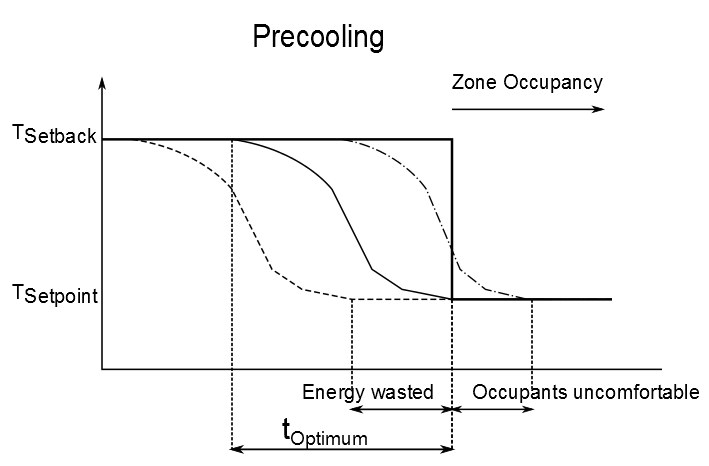
\includegraphics[width=0.9\textwidth, height=0.9\textheight, keepaspectratio=true]{media/image6731.png}
\caption{Optimal Start Control \protect \label{fig:optimal-start-control}}
\end{figure}

In practice a few proprietary algorithms are used to predict this start time value for preheating and precooling operation. ASHRAE Handbook refers to work done by (Seem, Armstrong, \& Hancock, 1989) which compares seven different equations and suggests a set of equations for preheating and precooling time prediction.

\subsubsection{Algorithms}\label{algorithms}

There are a few algorithms to predict the start time for the HVAC system. Among these algorithms following are the promising ones that can be implemented in a simulation environment.

\subsubsection{Constant Start Time}\label{constant-start-time}

This is the simplest format of the optimum start algorithm. The HVAC system will start the HVAC system at a fixed number of hours before occupancy as specified by the user.

\subsubsection{Constant Temperature Gradient}\label{constant-temperature-gradient}

In practice most of the HVAC control manufacturers use a temperature gradient as a thermal capacity factor, in which temperature rise per unit time i.e. °C/hour is measured for the unoccupied building and then the difference between space temperature and set-point temperature is divided by this factor to calculate the actual number of hours before occupancy are needed to start the HVAC system.

\subsubsection{Adaptive Temperature Gradient}\label{adaptive-temperature-gradient}

Adaptive control is used to modify the temperature gradient depending on the time required to meet the set-point on the prior days. The adaptive algorithm takes the arithmetic average of the actual temperature gradients calculated for the specified number of previous days.

\subsubsection{Adaptive ASHRAE Algorithm}\label{adaptive-ashrae-algorithm}

The equations suggested in the ASHRAE Handbook are used in combination with a recursive linear least square method to determine the optimum start/recovery time empirically. Depending on heating or cooling operation the start time is categorized as preheating or precooling time. According to (Seem, Armstrong, \& Hancock, 1989) the preheating time is a strong function of outdoor temperature whereas precooling time is not strong function of outdoor temperature if space temperature is close or less than the setback temperature. Thus, two different equations are suggested for preheating and precooling time.

For precooling time:

\begin{equation}
{t_i} = {a_0} + {a_1}{T_{z,i}} + {a_2}T_{z,i}^2
\end{equation}

For preheating time:

\begin{equation}
{t_i} = {a_0} + \left( {1 - {w_i}} \right)({a_1}{T_{z,i}} + {a_2}T_{z,i}^2) + {w_i}{a_3}{T_{o,i}}
\end{equation}

where, on \emph{i}\(^{th}\) day:

\(t_{i}\) is the start/recovery time

\(T_{z,i}\) is the zone temperature

\(T_{o,i}\) is the outdoor temperature

\(w_{i}\) is a weighting factor which determines weighting given to outside and zone temperature:

\begin{equation}
{w_i} = {1000^{ - \frac{{\left( {{T_{z,i}} - {T_{unocc}}} \right)}}{{\left( {{T_{occ}} - {T_{unocc}}} \right)}}}}
\end{equation}

where \(T_{unocc}\) and \(T_{occ}\) are setpoint temperatures during unoccupied (setback) and occupied periods, respectively.

Coefficients \emph{a\(_{0}\), a\(_{1}\), a\(_{2}\)} (and \emph{a\(_{3}\)}) are separately calculated for heating and cooling operation and are updated from the optimum times from last three days thus; these coefficients carry history and adapt the trend from previous days.

The optimum time for past days is determined using:

\begin{equation}
{t_{opt,\left( {i - 1} \right)}} = {k_{\left( {i - 1} \right)}}\Delta t - \Delta t\left( {1 - \frac{{{q_{\left( {i - 1} \right)}}}}{{{q_{max}}}}} \right)
\end{equation}

where:

\emph{k} are the time steps required for recovery

\({\Delta t}\) is the time-step

\(t_{opt,(i-1)}\) is the recovery time on (\emph{i}-1)\(^{th}\) day

\(q_{(i-1)}\) is the energy extracted or added during last time step

\(q_{max}\) is the maximum capacity of the equipments.
